% \section{Methods}

Our model groups individuals based on disease status (Susceptible, Infectious or Recovered) and testing status (\emph{untested}, waiting-for-\emph{positive}, waiting-for-\emph{negative}, or \emph{confirmed positive}) (\fref{fig:flowchart}).  The testing status of an individual in a given disease compartment $X$ (where $X \in \{S,I,R\}$) is denoted by a subscript, namely $X\_u$, $X\_p$, $X\_n$ and $X\_c$, for \emph{untested}, waiting-for-\emph{positive}, waiting-for-\emph{negative}, or \emph{confirmed positive}, respectively.  Two `accumulator' compartments, $N$ and $P$, are included in order to collect cumulative reported negative or positive tests. The model equations \eqref{model} and details of calculation of the basic reproduction number $\Rnum$ are presented in \appref{R0}.

\begin{figure}
\begin{center}
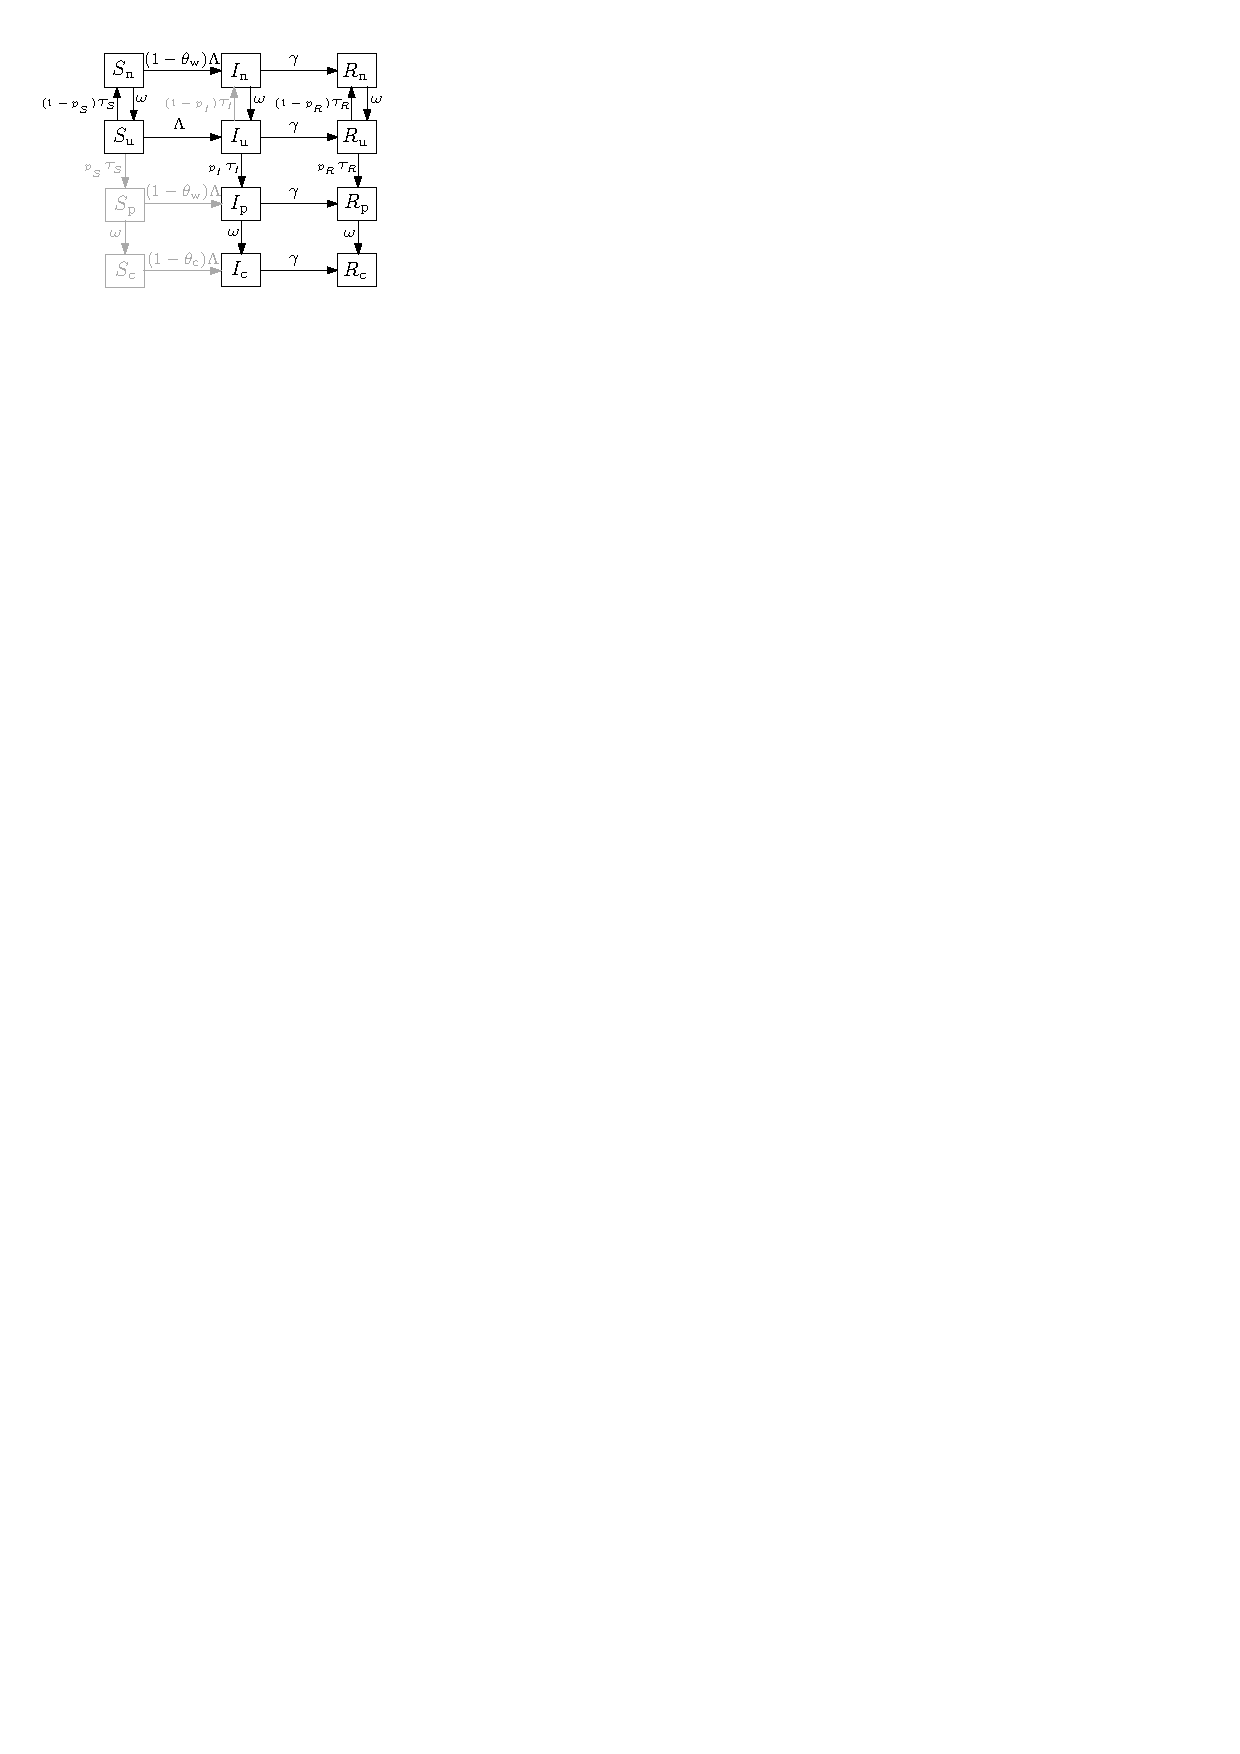
\includegraphics[scale=1.5]{pix/sir_comp.pdf}
\caption{\small Flowchart of the SIR (Susceptible-Infectious-Recovered) model, \ref{model}. The disease-based status of a compartment $X$ ($X \in \{S,I,R\}$) is combined with the testing status including $X\_u$, $X\_p$, $X\_n$ and $X\_c$, for \emph{untested}, waiting-for-\emph{positive}, waiting-for-\emph{negative}, or \emph{confirmed positive}, respectively. The force of infection is denoted by $\Lambda$ (Eq.~\eqref{Lambda}); $\gamma$ is the recovery rate; $\omega$ is the rate of test return; and \testing{X} (Eq. \eqref{test}) and $p_X$ represent the \percap testing rate and the sensitivity (probability of positive tests), respectively, for compartment $X$. For further description of the parameters see Table~ \ref{tab:params}.
Note that there is a slight mismatch in the top-to-bottom order of the testing-based compartments of each disease-based compartment $X$ between this flowchart and the model equations \eqref{model}; here we have switched  $X\_u$ and $X\_n$ for visual clarity.
\label{fig:flowchart}}
\end{center}
\end{figure}

Table~\ref{tab:params} defines the model parameters, which are generally \percap flows between compartments, or modifiers to these flow rates. The novel component of the model lies in the compartment-specific relative testing weights $w_S$, $w_I$ and $w_R$; these give the relative rates at which people in the $S$, $I$, and $R$ compartments are tested, respectively. Thus, we can specify different levels of testing focus from random (all weights equal) to highly targeted (higher weights in more intensively tested compartments). For example, $w_I/w_S=3$ means that infected individuals are tested at three times the \percap rate of susceptible individuals. 

In order to allow parameterization of the model by the total (overall) \percap testing rate, we define the weighted size of the testing pool $W = w_S S\_u + w_I I\_u + w_R R\_u$, and calculate a scaling parameter for testing as:
\begin{equation}
\label{sigma}
\sigma = \frac{\rho N}{W},
\end{equation}
where $\rho$ is the \percap testing intensity for the population, defined as the number of daily tests administered in a population of size $N$.
Thus, the \percap testing rate for compartment $X \in \{S,I,R\}$ is 
\begin{equation}
\label{test}
\testing{X}=\sigma w_X.
\end{equation}
For a highly sensitive test, infected people typically flow through to the ``confirmed positive'' ($I\_c$, $R\_c$) compartments and are thus not considered for further testing. Over the course of the epidemic, a sufficiently large fixed testing rate as specified in \eqref{sigma} can exhaust the pool of people available for testing, leading to a singularity when too few people are left untested to support the specified rate. Although this phenomenon does not affect our analysis of $\Rnum$, it can affect model dynamics (we present an adjustment to the model that solves this problem in \appref{singularity}).

The classical SIR model assumes a well-mixed population; homogeneity of the population (i.e., all individuals are equally susceptible and equally infectious with the same recovery rate when infected); exponentially distributed duration of infection; and large population size \citep{keeling2011modeling}. In addition to these standard assumptions, our model assumes: 
\begin{enumerate}[(i)]
\item there is a single force of infection (new infections per unit time per susceptible), $\Lambda$, defined as
  \begin{equation}
  \label{Lambda}
  \Lambda=\frac{\beta}{N} \big(I\_u + (1-\theta\_w)(I\_n+I\_p) + (1-\theta\_c)I\_c \big),
  \end{equation}
with transmission rate $\beta$; $\theta\_w$ is the isolation efficacy (reduction of the probability of transmission) for individuals waiting for test results, while $\theta\_c$ is the isolation efficacy for individuals who have received a ``confirmed'' positive test (Table~\ref{tab:params}). Susceptible individuals who are waiting for test results experience an additional transmission reduction factor of $1-\theta\_w$ (\fref{fig:flowchart}). 
\item confirmed-positive individuals isolate at least as effectively as those awaiting test results, i.e.,
$$0\leq\theta\_w\leq\theta\_c\leq 1.$$ 
\end{enumerate}
For simplicity we assume that tests are perfectly \emph{specific} --- uninfected individuals never test positive ($p_s=0$). Thus there are no waiting-for-positive or confirmed-positive susceptible individuals, which reduces the number of model states from 12 to 10.

\begin{table}[htp]
\centering
%%\begin{tabular}{|c|L{2in}cc|} \hline
%% making use of ragged2e and array packages:
{\RaggedRight
\begin{tabular}{ c | m{6cm} | c | c }
  \textbf{Symbol} & \textbf{Description} & \textbf{Unit} & \textbf{Value} \\ \hline
  $N$     & Total population size & people & $10^6$ \\ \hline
  $\omega$  & Rate of test return, i.e., rate of onward flow from ``waiting'' to ``confirmed'' or ``untested'' compartments  & 1/day & - \\ \hline
  $\gamma$ & Recovery rate & 1/day & 1/6 \\ \hline 
  $\rho$   & \percap testing intensity & 1/day & - \\ \hline 
  $\theta\_w$ & Isolation efficacy (reduction of the transmission probability) for ``waiting'' individuals & - & - \\ \hline
  $\theta\_c$ & Isolation efficacy for ``confirmed positive'' individuals & - & -  \\ \hline
  $\beta$ & Transmission rate & 1/day & 0.5 \\ \hline
  $\Lambda$ & Force of infection & 1/day & - \\ \hline
  $p_S$ & Probability of positive tests for $S$ ($= 1-\textrm{specificity}$) & - & 0 \\ \hline
  $p_I$ & Probability of positive tests for $I$ ($= \textrm{sensitivity}$) & - & 1 \\ \hline
  $p_R$ & Probability of positive tests for $R$ ($= 1-\textrm{specificity}$) & - & 0.5 \\ \hline
  $w_S, w_I, w_R$ & Relative testing weights & - &
  \begin{minipage}[t]{0.21\columnwidth}%
    Random:~$\{1,1,1\}$ \\ Targeted:~$\{0.3,1,1\}$
  \end{minipage} \\
  %%\hline
\end{tabular}
} % end \RaggedRight
\caption{\label{tab:params}Parameters of the model specified  by the flow chart in \fref{fig:flowchart} and equations~\eqref{model}.}
\end{table}

The Disease-Free Equilibrium (DFE) for the expanded SIR model (Eqs.~\ref{model}) is found by setting the infected compartments to 0 and solving for the unknowns. The DFE is
\begin{equation}
\label{dfe}
S\_n^*= \frac{\rho}{\omega} N, \ S\_u^*= N-S_n^*, \text{~and~} I_j=R_j=0 \ \text{for all }j.
\end{equation}
The corresponding \percap testing rate (Eq.~\ref{test}) for the infected compartment $I$ at DFE is one of the key analysis parameters and can be simplified as 
\begin{equation}
\label{eq:fi}
\testinghat{I} = (\omega\rho/(\omega-\rho))w_I/w_S \quad .
\end{equation}

The basic reproduction number, $\Rnum$, was calculated by using the next-generation matrix method \citep{van2002reproduction}. We write $\Rnum$ as
\begin{equation}
\label{R0}
\Rnum= \frac{\beta}{\gamma} \left(1-\Delta\right), 
\end{equation}
where $\beta/\gamma$ is the classical value for a simple model \citep{keeling2011modeling}, and $1-\Delta$ is the proportional reduction due to testing and isolation processes. $\Delta$ therefore measures the ``effectiveness of control'': how much these processes in reducing spread from low levels, and is in turn given by:
\begin{equation}
  \label{eq:del4a}
  \Delta= \frac{1}{C N}\big(C_1 S\_u^*+(C_2(1-\theta\_w)+C \theta\_w)S\_n^*\big),
\end{equation}
where
\begin{align}
\label{eq:C12}
C_{\phantom 1} &= (\omega+\gamma) \Big(\gamma(\omega+\gamma)+(\gamma+\omega p_I)\testinghat{I}\Big),\\
C_1 &= (\omega+\gamma)(\theta\_w \gamma+\theta\_c \omega p_I) \testinghat{I},\\
C_2 &= \Big( \omega\gamma(1+p_I)\testinghat{I}+\gamma^2(\omega+\gamma+\testinghat{I})\Big)\theta\_w + \omega^2p_I \testinghat{I} \theta\_c.
\end{align}
(\appref{R0} gives a detailed derivation of these expressions.)
This explicit formula enables us to study the effects of testing and isolation parameters on $\Rnum$ both analytically and via numerical solutions.
We are specifically interested in parameters that could be manipulated by public health policy: isolation efficacy, $\theta\_c$ and $\theta\_w$; \percap testing intensity, $\rho$; and the rate of test return, $\omega$. In particular, we look at the partial derivatives of $\Delta$ with respect to these parameters (Appendices~\ref{app:rho} and \ref{app:omega}). 
We derived general expressions for these derivatives. However, we analyzed the effect of $\omega$ on $\Delta$ for the special case of low testing intensity. Specifically, by making the restriction $\rho \ll 1$, we are able to Taylor-expand $\Delta$ at $\rho=0$, use the linear approximation with respect to $\rho$ and analyze the resulting simplified derivatives to illustrate a surprising non-monotonic relationship between $\Delta$ and $\omega$. 

Analytic calculation of the next-generation matrix and simplification of the $\Rnum$ expression, were performed in Maple\textsuperscript{\texttrademark} \citep{maple14}; numerical calculation and contour plots were done in R \citep{r}.
We computed the values and contours of $\Delta$ at both low (\fref{pan}) and high (\fref{pan2}) testing intensities, and for both random testing ($w_S=w_I=w_R=1$) and targeted testing ($w_S=0.3$; $w_I=w_R=1$). Because it is expressed as a proportion of $\Rnum$, the effectiveness of control $\Delta$ is (at least in the $\rho \ll 1$ case, Eq.~\ref{eq:lin}) independent of the transmission rate $\beta$, and hence of $\Rnum$ in the case where we vary $\Rnum$ by changing the transmission rate for a fixed generation interval.

The low-testing case (\fref{pan}) reflects the case where testing intensity $\rho$ is small relative to the population size. Specifically, $\rho \in [0,0.013]$, and test return rate $\omega\in [1/12,2]$. This testing intensity is of the correct order of magnitude (although typically larger than) testing rates during the \covid pandemic, i.e., a maximum of 1.3\% of the population per day (approximately four times the maximum testing rate in Ontario, Canada in mid-2021). The less realistic high-testing case (\fref{pan2}) is included to highlight the occurrence of non-monotonic changes in $\Rnum$ with respect to $\rho$.
In \fref{pan2} the maximum capacity of $\rho$ is larger relative to the population size, $\rho \in [0,1/5)$ and the test return rate $\omega\in [1/5,2]$; these values are clearly unrealistic for a large population but might be relevant for small populations undergoing focused testing, such as a sports league or university. In these figures, the implied baseline reproduction number (for the SIR model without testing) is $\Rnum=\frac{\beta}{\gamma}=3$.  The different ranges of test return rates $\omega$ for the cases of low and high testing intensities is due to the restriction $\rho<\omega$, which is a requirement for a feasible DFE (\ref{dfe}).
  